\chapter{Appendix Case Studies}
\label{chap:appendix1}


\begin{figure}
\centering
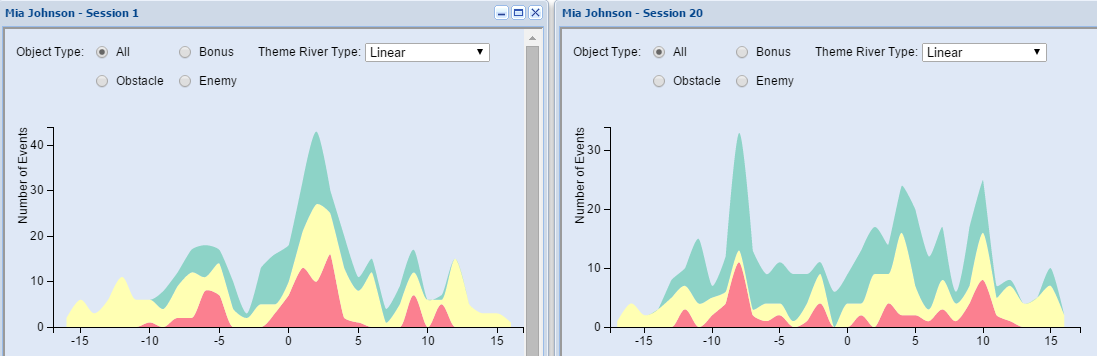
\includegraphics[width=140mm]{appendix_case1_compare_session_stackedgraph.png}
\caption{Stacked Graph comparison of Session 1 and Session 20}
\label{fig:app1_stacked}
\end{figure}

\begin{figure}
\centering
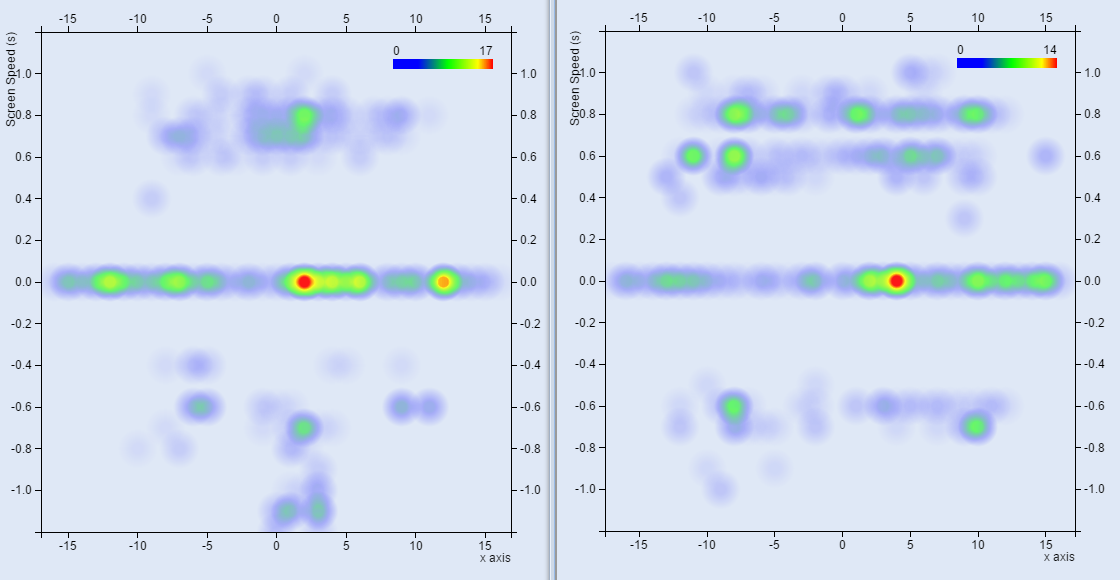
\includegraphics[width=140mm]{appendix_case1_compare_session_heatmap.png}
\caption{Heatmap comparison of Session 1(left) and Session 20(right)}
\label{fig:app1_heatmap}
\end{figure}

\begin{figure}
\centering
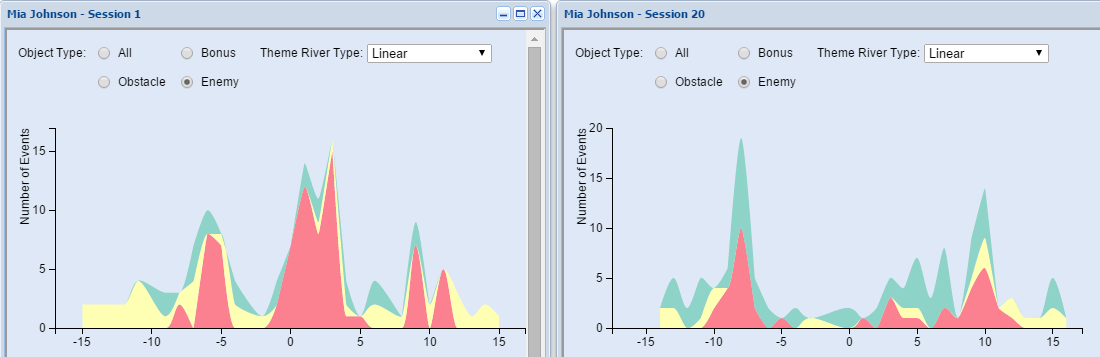
\includegraphics[width=140mm]{appendix_case1_compare_session_stackedgraph_enemy.png}
\caption{Stacked Graph comparison of Session 1 and Session 20 for Enemy}
\label{fig:app1_stacked_enemy}
\end{figure}

\begin{figure}
\centering
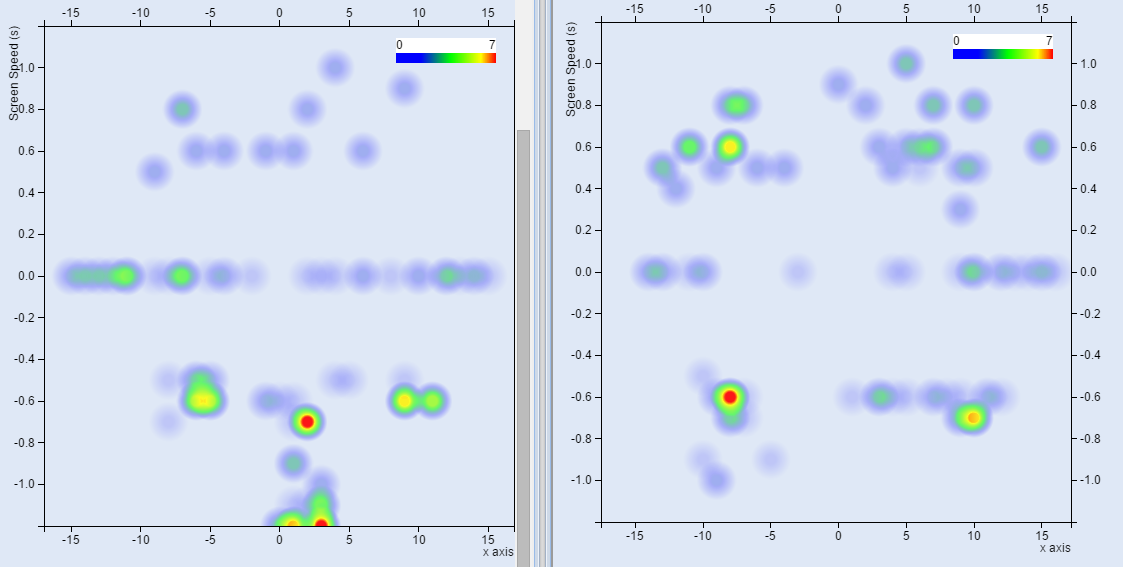
\includegraphics[width=140mm]{appendix_case1_compare_session_heatmap_enemy.png}
\caption{Heatmap comparison of Session 1(left) and Session 20(right) for Enemy}
\label{fig:app1_heatmap_enemy}
\end{figure}

\begin{figure}
\centering
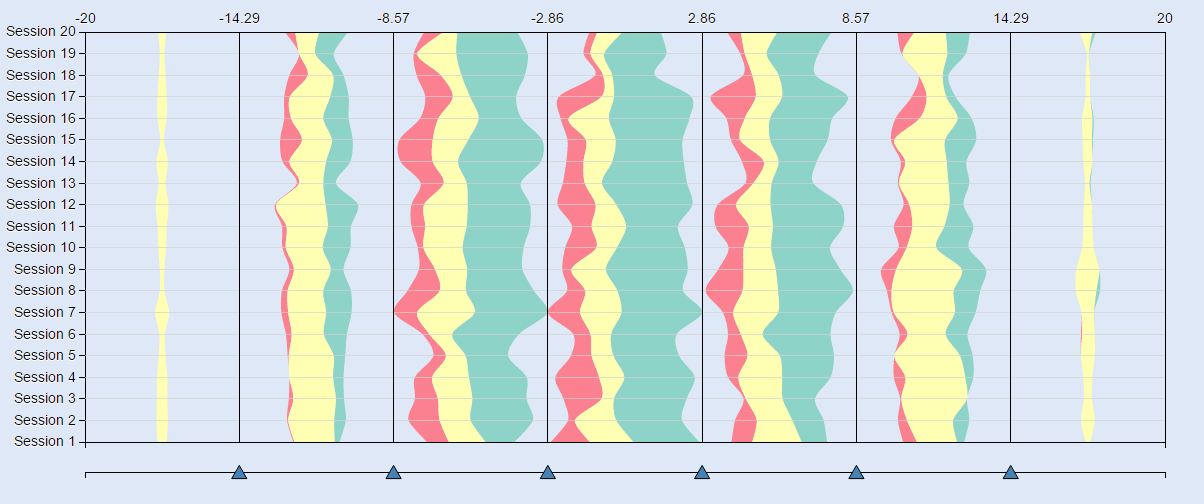
\includegraphics[width=140mm]{case1_type1.png}
\caption{Summary Visualization by x-range}
\label{fig:case1_type1}
\end{figure}

\begin{figure}
\centering
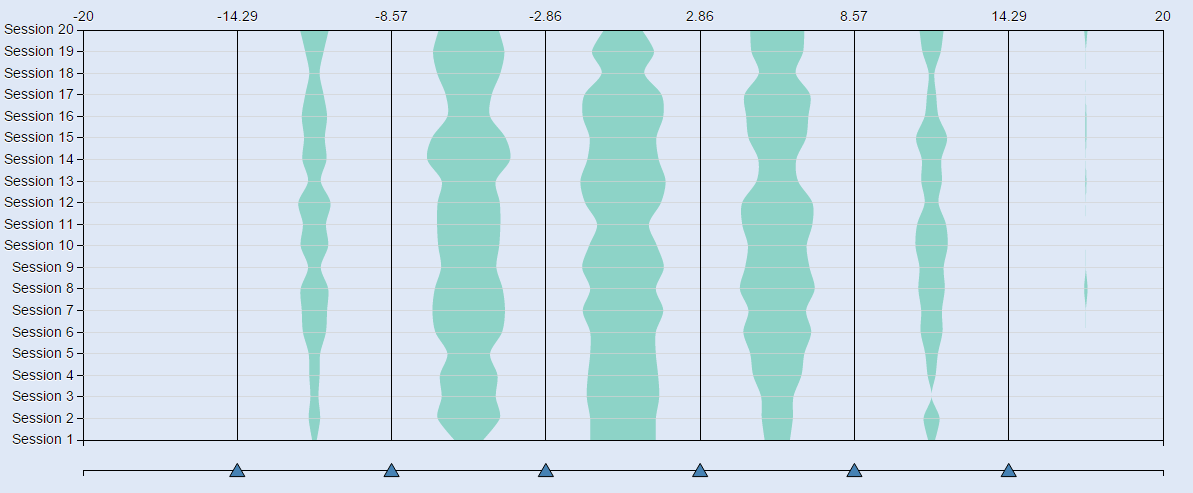
\includegraphics[width=140mm]{case1_type1_select.png}
\caption{Summary Visualization by x-range, filtered for positive events}
\label{fig:case1_type1_select}
\end{figure}

\begin{figure}
\centering
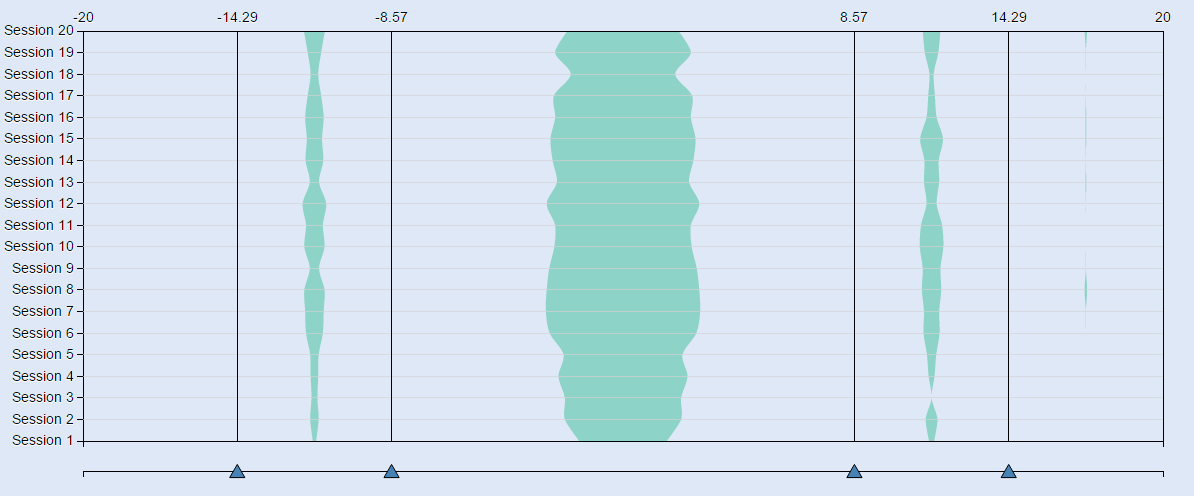
\includegraphics[width=140mm]{case1_type1_select_clustered.png}
\caption{Summary Visualization by x-range, filtered for positive events and clustered}
\label{fig:case1_type1_select_c}
\end{figure}

\begin{figure}
\centering
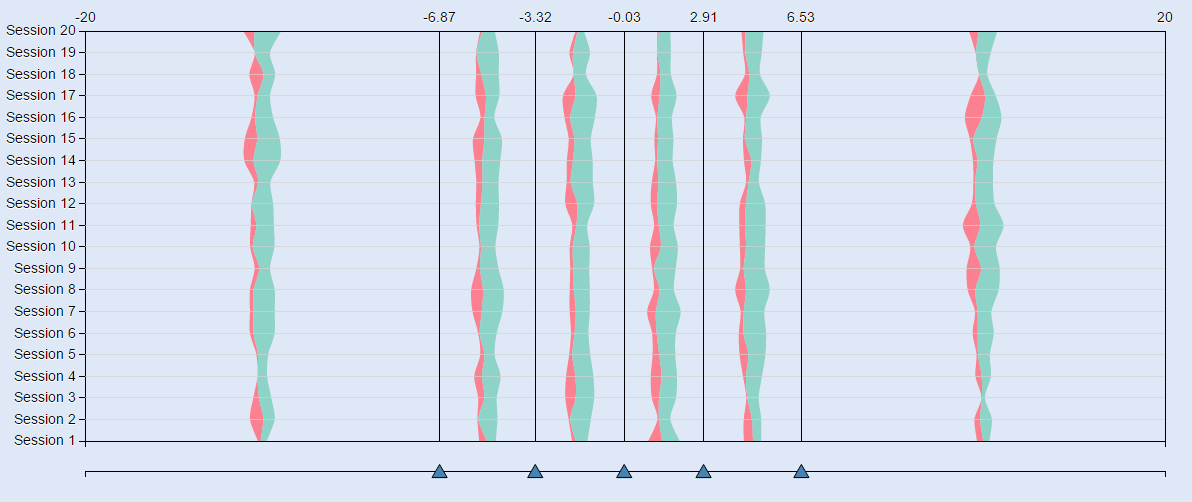
\includegraphics[width=140mm]{case1_type2.png}
\caption{Summary Visualization by number of events, filtered for positive and negative events}
\label{fig:case1_type2}
\end{figure}

\begin{figure}
\centering
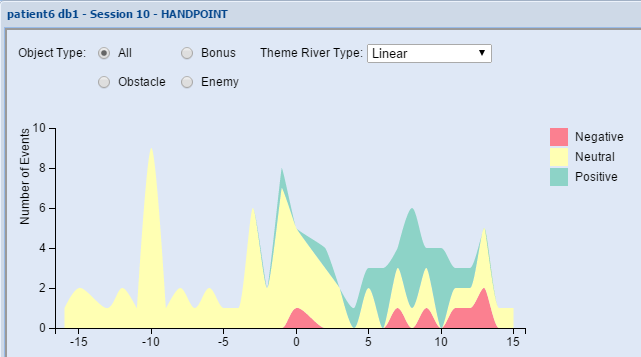
\includegraphics[width=140mm]{case2_stacked.png}
\caption{Stacked Graph of Session 10}
\label{fig:case2_stacked}
\end{figure}

\begin{figure}
\centering
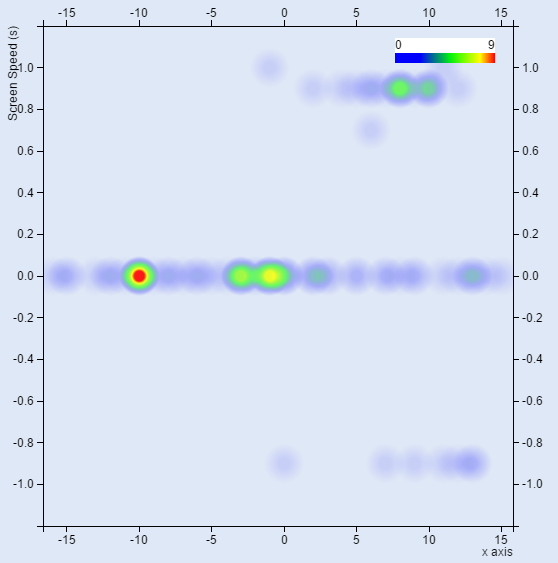
\includegraphics[width=100mm]{case2_heatmap.png}
\caption{Heatmap of Session 10}
\label{fig:case2_heatmap}
\end{figure}

\begin{figure}
\centering
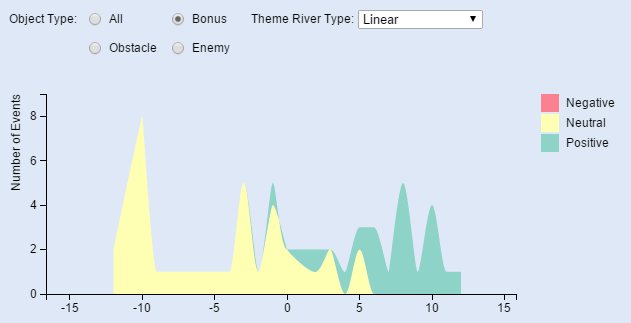
\includegraphics[width=140mm]{case2_stacked_bonus.png}
\caption{Stacked Graph of Session 10, filtered by bonus}
\label{fig:case2_stacked_bonus}
\end{figure}

\begin{figure}
\centering
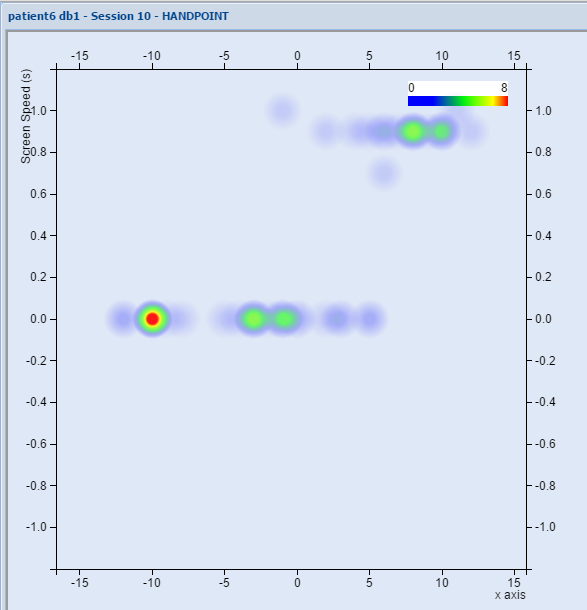
\includegraphics[width=100mm]{case2_heatmap_bonus.png}
\caption{Heatmap of Session 10, filtered by bonus}
\label{fig:case2_heatmap_bonus}
\end{figure}

\begin{figure}
\centering
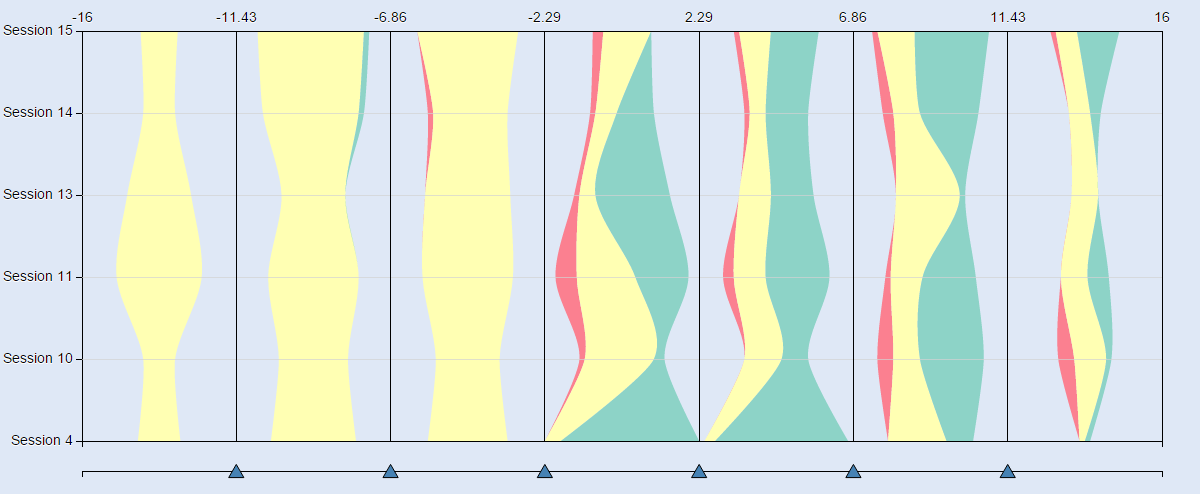
\includegraphics[width=140mm]{case2_summary.png}
\caption{Summary visualization of Patient 6}
\label{fig:case2_summary}
\end{figure}

\begin{figure}
\centering
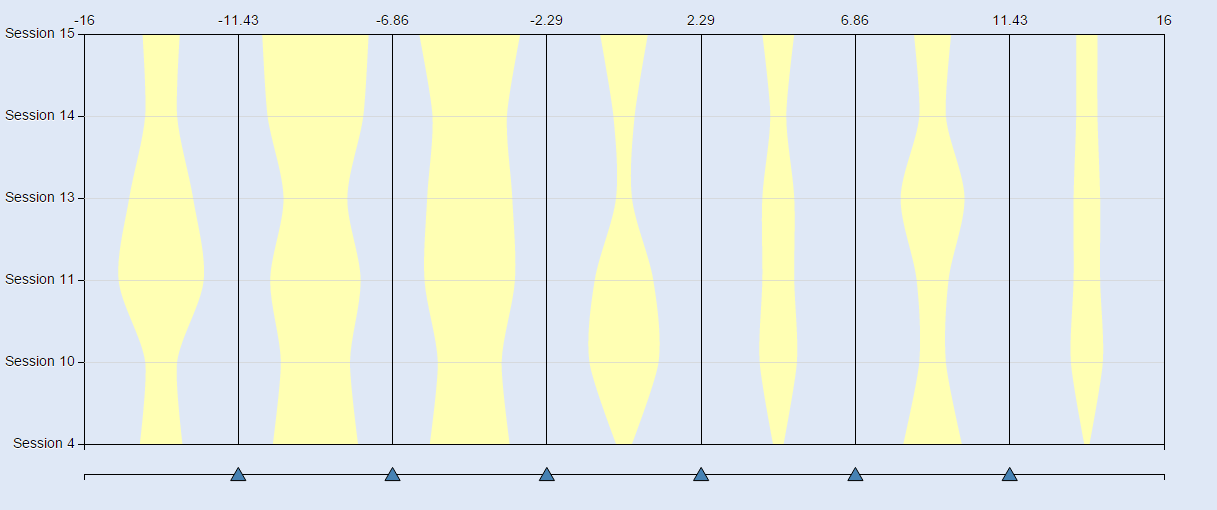
\includegraphics[width=140mm]{case2_summary_neutral.png}
\caption{Summary visualization of Patient 6, filtered by neutral events}
\label{fig:case2_summary_neutral}
\end{figure}

\begin{figure}
\centering
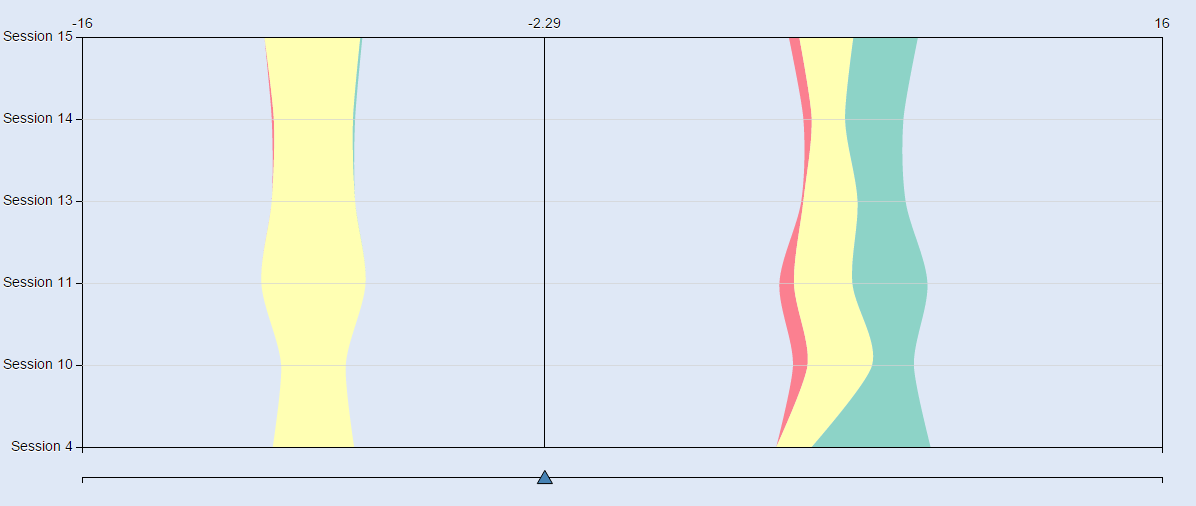
\includegraphics[width=140mm]{case2_summary_clustered.png}
\caption{Summary visualization of Patient 6, clustered}
\label{fig:case2_summary_clustered}
\end{figure}

\begin{figure}
\centering
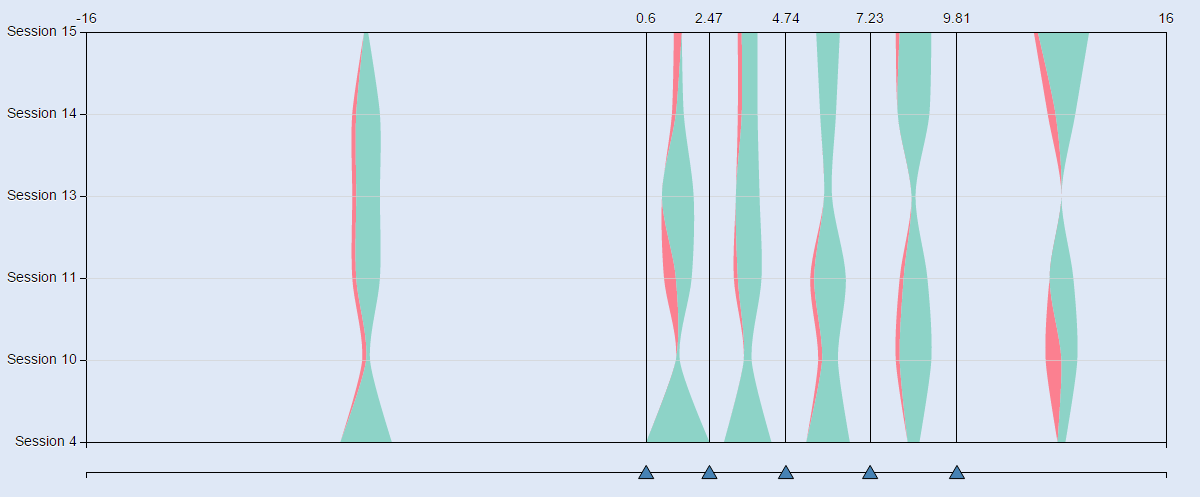
\includegraphics[width=140mm]{case2_summary_type2.png}
\caption{Summary visualization of Patient 6 with sections divided by number of events, filtered by positive and negative events}
\label{fig:case2_summary_type2}
\end{figure}